創造一組樣本大小為5,連續抽20組subgroups)的標準常態隨機樣本。

\begin{lstlisting}[language=R]
    > data <- matrix(rnorm(100), 20, 5)
    > print(round(data, 3))
            [,1]   [,2]   [,3]   [,4]   [,5]
     [1,]  2.043 -0.275 -1.099  1.788  1.146
     [2,] -0.381  1.725  0.272  0.214 -1.298
     [3,]  0.717 -2.442 -0.583 -0.465 -1.055
     [4,] -0.968 -0.247  0.600 -0.478  0.889
     [5,]  0.477 -1.528 -0.480 -1.355  0.164
     [6,]  0.964 -1.084  0.273  0.637  0.574
     [7,]  2.933  0.862 -0.627  0.343  0.447
     [8,] -0.893 -0.304 -1.352  1.137  0.302
     [9,]  1.463 -1.359  0.671  0.260 -0.387
    [10,]  0.612 -0.675 -0.390 -1.919 -0.581
    [11,] -1.102  1.293  1.017 -1.831 -0.886
    [12,]  0.194 -0.681 -0.417  0.196  0.878
    [13,] -0.032  1.570 -0.799 -1.416 -1.662
    [14,] -0.638 -0.806  1.302  0.263  0.154
    [15,]  0.905  0.518 -1.302  0.201 -2.116
    [16,] -0.067 -1.010  0.291 -0.493 -0.280
    [17,] -0.941  0.233  0.069  0.181 -0.193
    [18,]  0.379  1.565  1.353  0.330  0.086
    [19,]  2.447 -0.192 -1.132  0.352  0.124
    [20,] -0.283  0.764 -0.801 -0.618  0.352
\end{lstlisting}


(a) 計算各樣本組平均及全距。\\
    組平均:
        \begin{lstlisting}[language=R]
            > print(round(rowMeans(data), 3))
            [1] 0.721  0.106 -0.765 -0.041 -0.544  
            [6] 0.273  0.791 -0.222  0.130 -0.591 
            [11] -0.302  0.034 -0.468 0.055 -0.359
            [16] -0.312 -0.130  0.743  0.320 -0.117
        \end{lstlisting}
    組全距:
        \begin{lstlisting}[language=R]
            > for(i in 1:20){
                x[i]=max(data[i,])-min(data[i,])
                }
            > print(round(x, 3))
            [1] 3.143 3.022 3.159 1.857 2.005 
            [6] 2.048 3.560 2.489 2.822 2.531 
            [11] 3.124 1.559 3.232 2.108 3.021 
            [16] 1.302 1.174 1.478 3.578 1.566
            [1] 3.143 3.022 3.159 1.857 2.005 
            [6] 2.048 3.560 2.489 2.822 2.531 
            [11] 3.124 1.559 3.232 2.108 3.021 
            [16] 1.302 1.174 1.478 3.578 1.566
        \end{lstlisting}  

(b) 計算這20組樣本平均及全距。\\
    樣本平均:
        \begin{lstlisting}[language=R]
            > print(round(mean(rowMeans(data)), 3))
            [1] -0.034
        \end{lstlisting}
    樣本全距:
        \begin{lstlisting}[language=R]
            > print(round(mean(x), 3))
            [1] 2.439
         \end{lstlisting}
                
(c) 製程建立 $\Bar{x}$ 與 $R$ 管制圖。請問製程是否在統計管制內?
    \begin{lstlisting}[language=R]
        > q.xbar <- qcc(data , type = "xbar")
        > q.R <- qcc(data , type = "R")
    \end{lstlisting}
        
    $\Bar{x}$ chart:\\
    每個點皆有落在上下管制界線內,因此製程有在統計管制內受到控制。
            \begin{figure}[ht]
                \centering
                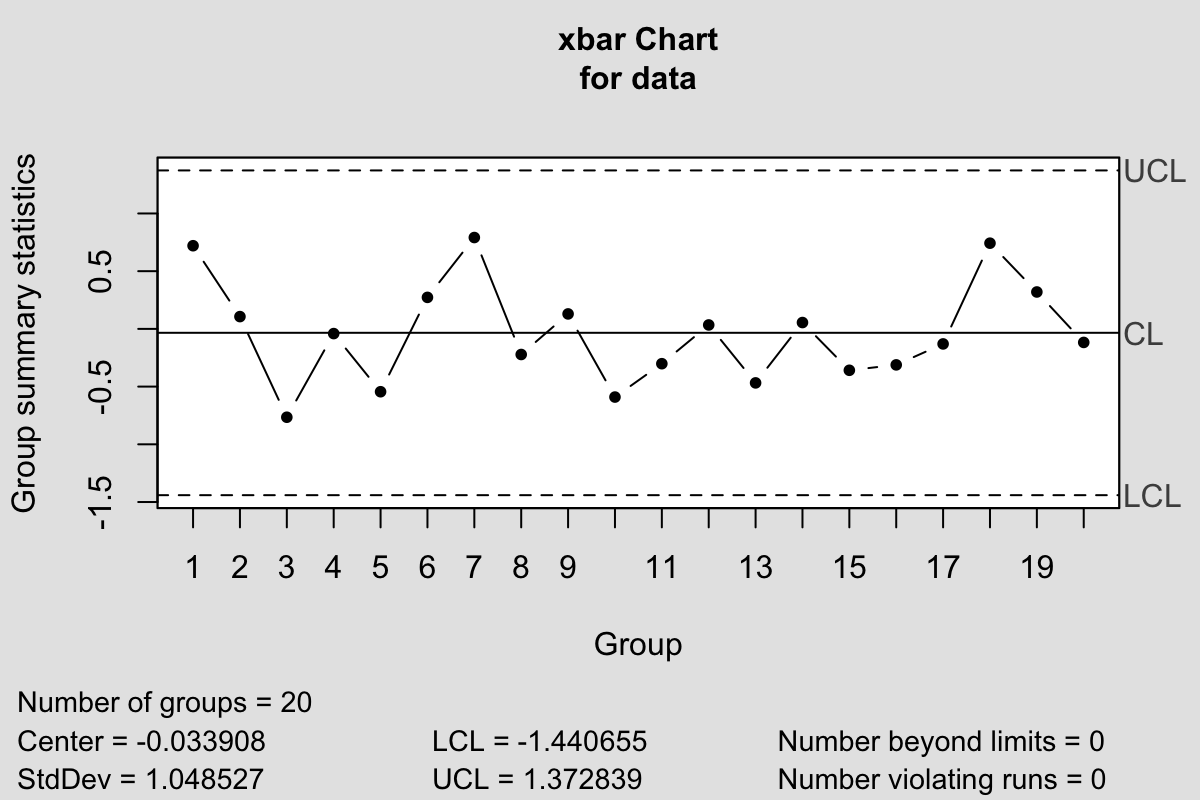
\includegraphics[width=10cm, height=7cm]{figures/Xbar_Chart.png}
                \caption{$\Bar{x}$ chart}
                \label{fig:1}
            \end{figure}
            
        \pagebreak
            
    $R$ chart:\\
    因為沒有數據在上下管制界線外,所以製程有受到控制。
            \begin{figure}[ht]
                \centering
                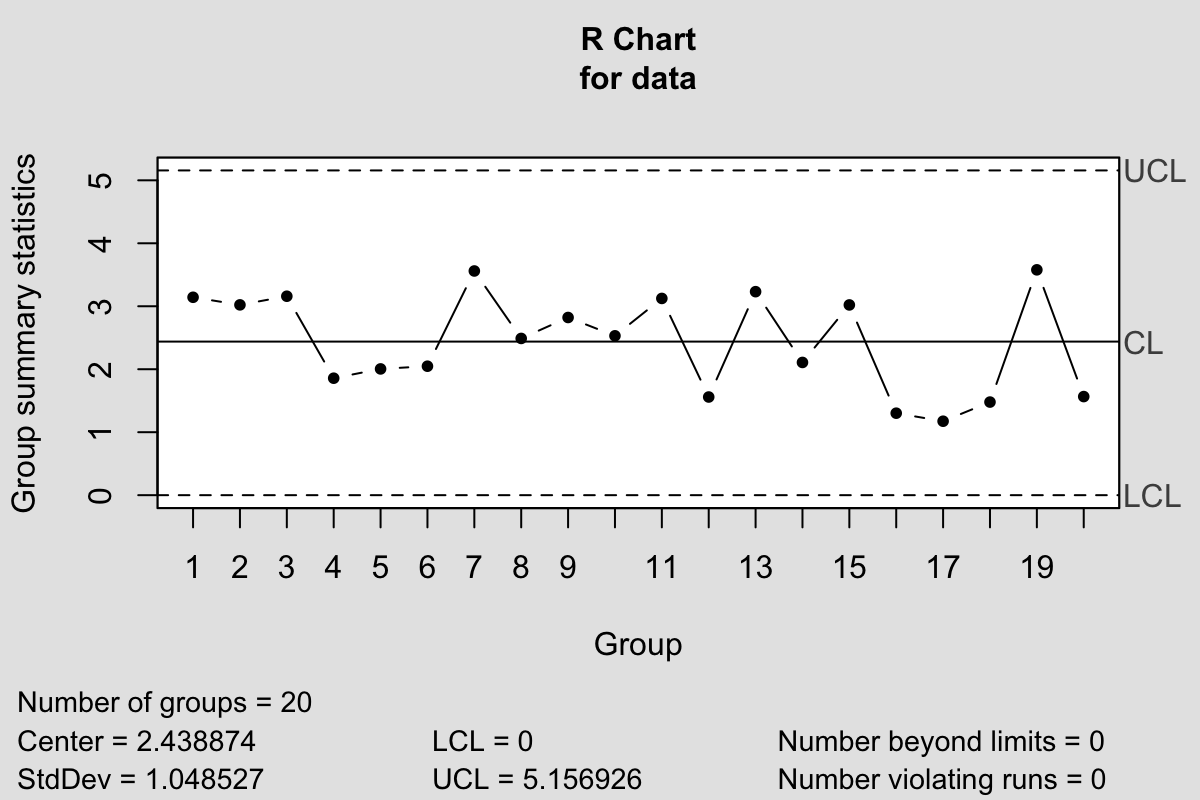
\includegraphics[width=10cm, height=7cm]{figures/R_Chart.png}
                \caption{$R$ chart}
                \label{fig:2}
            \end{figure}
        